% !TeX TXS-program:bibliography = txs:///biber
\documentclass[10pt,a4paper]{article}
\usepackage[T1]{fontenc}
\usepackage{graphicx}
\usepackage{mathtools}
\usepackage{amssymb}
\usepackage{amsthm}
\usepackage{thmtools}
\usepackage{xcolor}
\usepackage{nameref}
\usepackage{hyperref}
\usepackage{color}
%\usepackage[margin=1.5in]{geometry}
\usepackage{float}
\usepackage[
backend=biber,
style=authoryear,
natbib=true
]{biblatex}
\addbibresource{../bibliography.bib}


\title{\large EAE1223: Econometria III}
\author{\normalsize Exercícios sobre Decomposições de séries de tempo}
\date{}
\begin{document}
	\maketitle
	
	\paragraph{Parte 1} Faça o \textit{download} de \textbf{duas} séries de tempo de frequências mensal ou trimenstral. Alguns sítios úteis para encontrar dados: 
	\begin{enumerate}
		\item[a]  Sistema gerenciador de séries temporais, do BCB: \url{https://www3.bcb.gov.br/sgspub/};\footnote{Se preferir, você pode usar o pacote \texttt{dadosbc} para baixar as séries do SGS. A documentação do código está disponível em: \url{https://github.com/Figuera/dadosbc}. }
		\item[b] IPEA Data: \url{http://www.ipeadata.gov.br/};\footnote{Se preferir, você pode usar o pacote \texttt{ipeadatar} para baixar as séries do IPEA Data. A documentação do código está disponível em: \url{https://cran.r-project.org/web/packages/ipeadatar/vignettes/intro-ipeadatar.html}. }
		\item[c] FRED, do \textit{Federal Reserve} de Saint Louis: \url{https://fred.stlouisfed.org/}.
	\end{enumerate}
	Uma vez baixadas ambas as séries, responda as questões abaixo:
	\begin{enumerate}
		\item Para cada uma das séries, realize o ajuste sazonal manualmente (método das médias móveis centradas) e utilizando a metodologia Arima X13/Seats. Para cada variável, apresente em um gráfico os resultados obtidos e os dados sem ajuste. A série aparenta apresentar movimentos sazonais?
		\item Usando as séries dessazonalizadas via X13, extraia a tendência de cada série usando Filtro HP. Contraste a série com a tendência obtida. Você consegue identificar ciclos nos dados?
		\item Implemente a proposta de Hamilton para as suas séries. Quais as diferenças em relação ao filtro HP?
		
	
	\end{enumerate}
			\paragraph{Parte 2} Responda às questões abaixo:
			\begin{enumerate}
				\item[4] 		
				$$(1-\phi L) (1-L)y_t = \epsilon_t \, ,$$
				one $|\phi|<1$, e a sequência $\{\epsilon_t\}_t$ é independente e identicamente distribuída com média zero e variância finita. Encontre o componente cíclico da decomposição de Beveridge-Nelson de $y_t$. \textit{Dica:} $\mathbb{E}[\epsilon_s| y_{t}, y_{t-1}, y_{t-2}, \ldots ] = 0$ para todo $s > t$, pela hipótese de que a série $\{\epsilon_t\}_t$ é independente, e $\mathbb{E}[y_{s}| y_{t}, y_{t-1}, y_{t-2}, \ldots ] = y_t + \sum_{j=1}^s \mathbb{E}[\Delta y_{t+j}| y_{t}, y_{t-1}, y_{t-2}, \ldots ]$, para todo $s > t$.
				\item[5]  Os quadros abaixo apresentam diferentes medidas de ciclo, extraídas da série mensal de endividamento líquido do setor público brasileiro (como percentual do PIB), de janeiro de 2004 a dezembro de 2021. As medidas foram estimadas com dados de dezembro de 2001 a dezembro de 2021.
				\begin{figure}[H]
					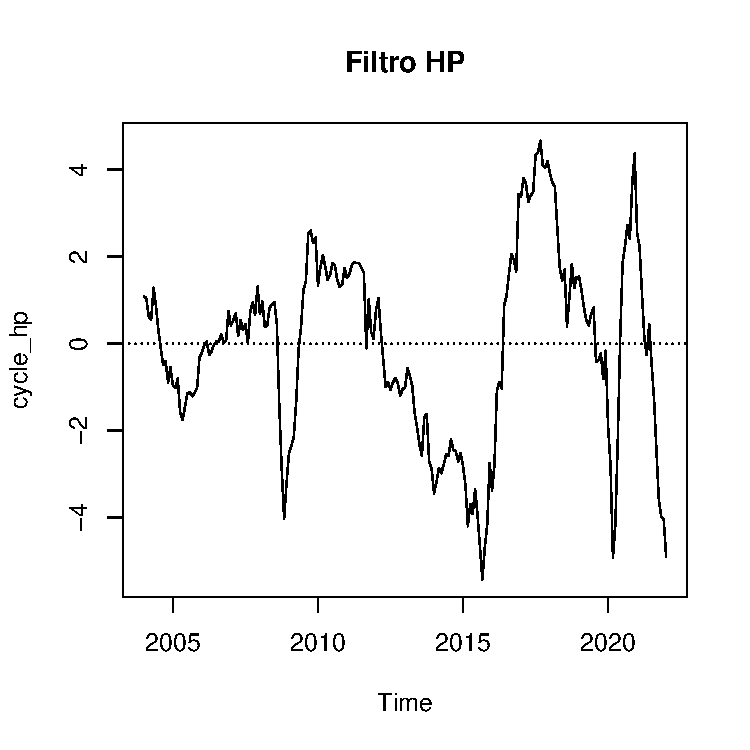
\includegraphics[scale=0.47]{hp.pdf}
					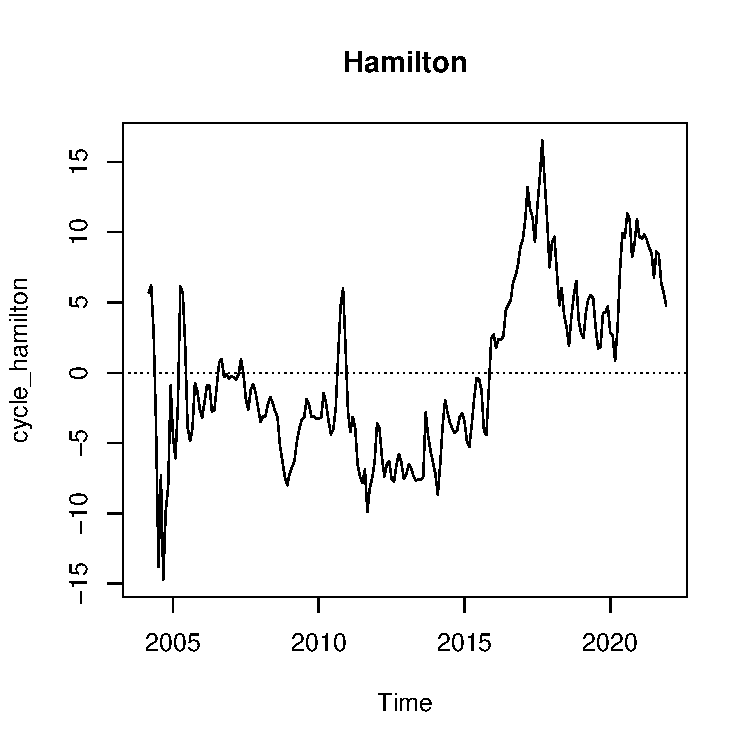
\includegraphics[scale=0.47]{hamilton.pdf}
					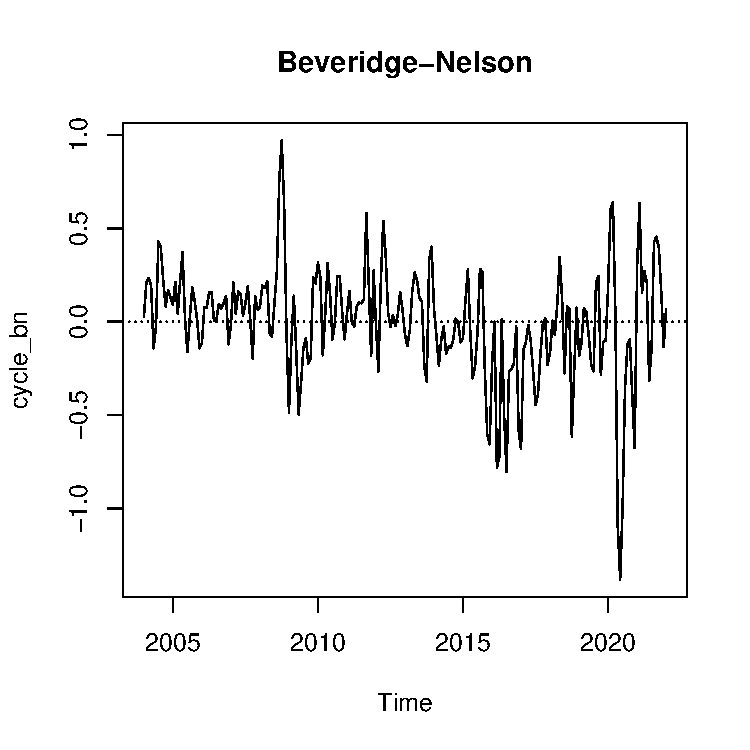
\includegraphics[scale=0.47]{bn.pdf}
				\end{figure}
				
				Explique as diferenças entre as medidas de ciclo observadas, à luz da metodologia de cada uma delas. Quais as vantagens e desvantagens do Filtro HP, em relação à proposta de Hamilton?
			\end{enumerate}
			
	
\end{document}